\section{WC 24/3/25}

\subsection*{Overview:}
This week was spent continuing my artifact development, spotting new improvements that can be made and features that can be easily added.

\subsection*{Achievements, Thoughts and Ideas:}
During my EPQ lesson this week I completed my Mid-Project Review within my PPR, this is an opportunity for me to evaluated my work so far and I am extremely proud of what I have achieved.

Some time was also spent this week mind mapping how the various tabs within my app should interact with each other.

Gathering feedback from my users is a vital aspect of my continued primary research and I didn't want to have to continually send different forms / surveys to them, so I spent some time researching feedback form best practices: \nameref{research:UserFeedbackGathering}(in addition to my research which aided the creation of my primary research survey) and making my own survey tab that can be easily accessed from the user dropdown menu.

\begin{figure}
    \centering
    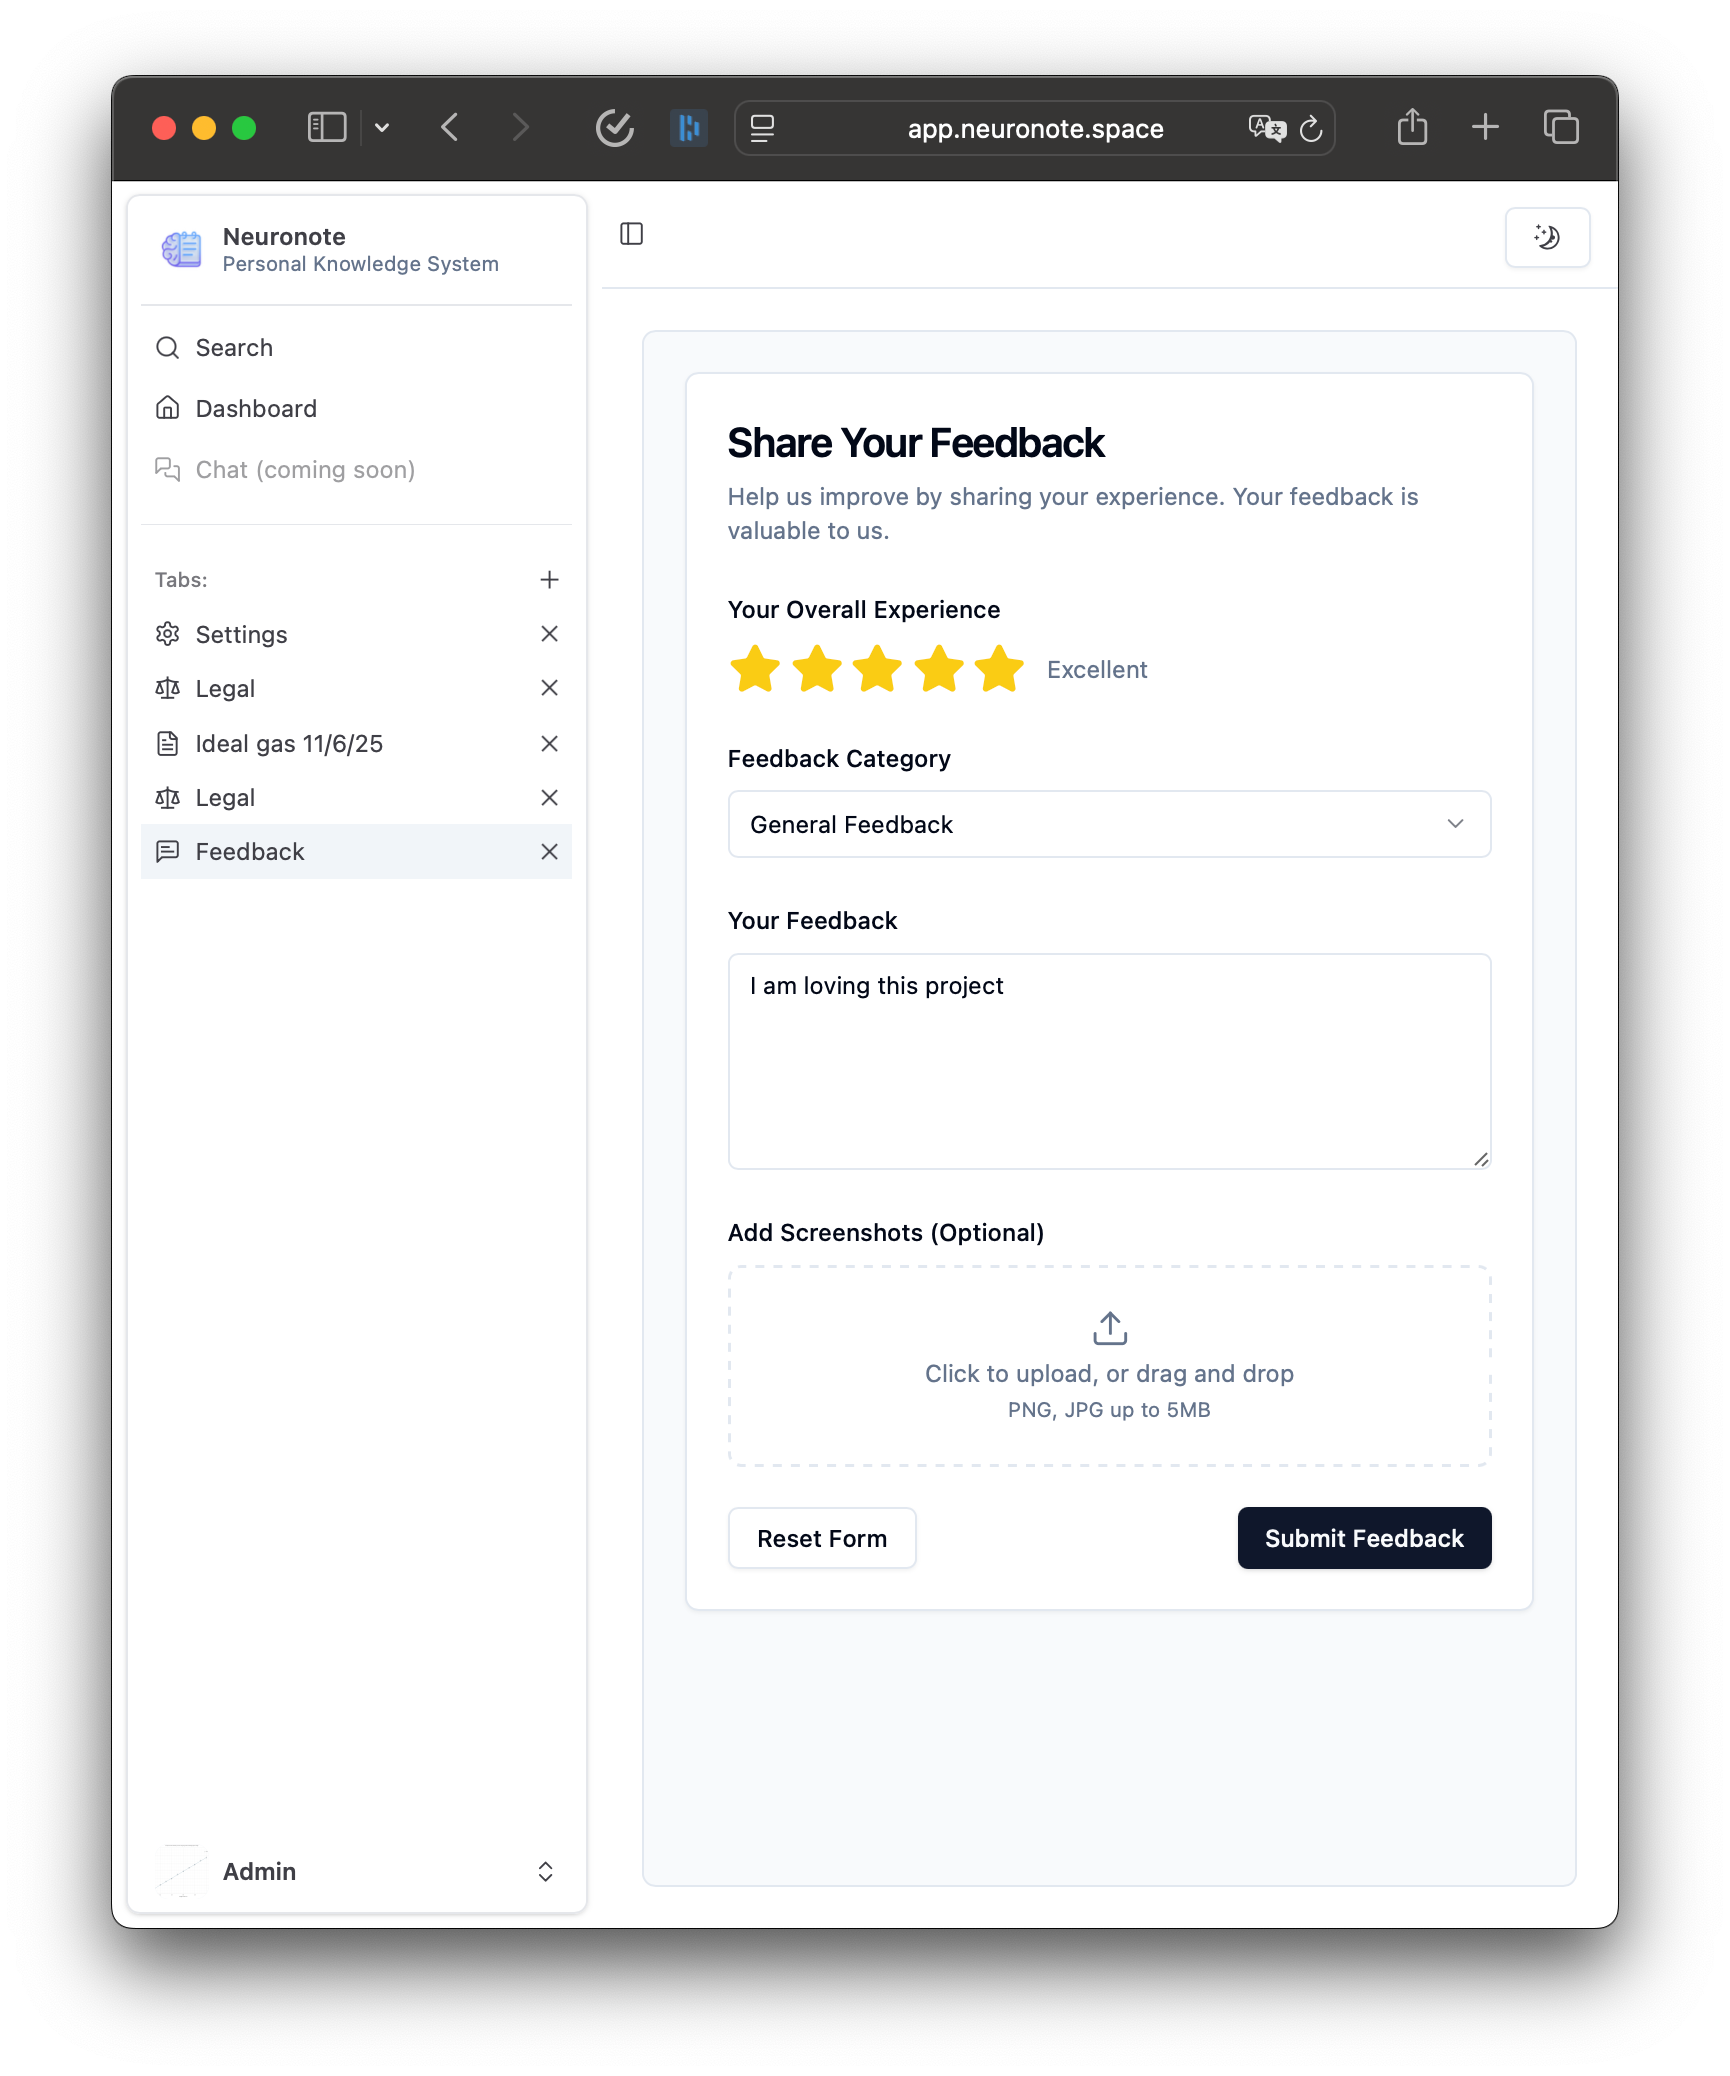
\includegraphics[width=0.6\textwidth]{Diary/23_WC_24-3-25/media/feedbackTab.png}
    \caption{Feedback Tab}
\end{figure}


Equally, I was now finding it frustrating having to change my app preferences (such as extensions on/off and hiding my personal information for screenshots) so I built I settings tab (though this has some work to do to make fully functional).

Please find both of my new tabs here: \nameref{prototype:SettingsAndFeedback}

I did spend some time building a system to store user media (such as photos, files and videos) in an efficient and easily searchable way however decided this would be out of scope of my EPQ but is something I definitely want to build in the future.

I ended up undoing some work I had done previously within my tab system. Previously when a note was selected and opened from the dashboard a new tab was opened showing the note (as expected), however when that note was closed the newly added tab switched to become a 'graph' tab showing all of the users notes. This resulted in many of these unused graph tabs being created and user confusion on how they were created. Now when a note is opened it opens purely as a note tab, if the note is closed then the tab is closed and the user is returned to the graph tab/dashboard that first opened the tab. Users can still add a graph view tab from the + on the side panel, this is useful for having multiple views of your note library each with their own filters. From now on I've decided the purpose of a tab should never change to prevent user confusion.

One change that I thought would be minor but was actually much more involved was the ability to add/remove/alter tags connected to a note within the document editor. Initially I tried to build this is a Tiptap extension (placing it within the 'note flow') however this faced issues when the tags connected to a note were changed externally (e.g. from the dashboard). In the end I made this an entirely separate component that is before the Tiptap note editor and placed the note name editor after it. This ensures it is easy/intuitive for a user to access but is always up-to-date. Please find this completed new feature here: \nameref{prototype:DocumentTagging}

\subsection*{Power of three?}
Here I would usually lay out daily tasks however I was now mainly working on many small tasks during my free time slots, these tasks are as below:

\textbf{Tasks:}

\begin{enumerate}
    \item Resource library of images files etc that can all be tagged \ding{55} - a good idea but on reflection out of scope of project
    \item Create settings tab \ding{51} (not fully functional)
    \item Research Feedback collection \ding{51}
    \item Create feedback Tab \ding{51}
    \item File folder view on left side \ding{51}
    \item Autosave every 5 seconds on note to prevent progress lost \ding{51}
    \item https://sachinmittal98.medium.com/how-to-add-a-copy-to-clipboard-button-in-tiptap-code-blocks-64ad32e357c7Ai \ding{55}
    \item summarise feature on right click / bubble menu and /ai block to ask question \ding{55}
    \item Utility tags such as type of resource, date created,  etc all usually hidden from view \ding{55}
    \item Auto capitalise first letter \ding{55}
    \item Recent notes - top 20 \ding{51}
    \item Fix bug loading on tab close \ding{51}
    \item Fix persisting preferences between loads \ding{51}
    \item Fix state on loads \ding{51}
\end{enumerate}

\subsection*{What went well?}
This week's work simplified many workflows for my app's users including myself. It is now much easier to navigate between different tabs and to easily open and create new notes

\subsection*{What was challenging?}
Some design elements took longer than I had initially planned for due to some unexpected complexities in software development however I identified improvements that were logical to make simultaneously as to minimise duplication of effort later on.


\subsection*{Plans for next week:}
Next week will be more implementation of my project.
